\documentclass{article}[]
\usepackage[textwidth=15cm]{geometry}
\usepackage[table,xcdraw]{xcolor}
\usepackage{graphicx}
\usepackage{listings}
\usepackage{hyperref}
\usepackage{pdfpages}
\usepackage{csvsimple}
\usepackage{float}
\usepackage{csquotes}
\makeatletter
\newcommand\urlfootnote@[1]{\footnote{\url@{#1}}}
\DeclareRobustCommand{\urlfootnote}{\hyper@normalise\urlfootnote@}
\makeatother

\begin{document}
\title{Neural Networks Assignment 2}
\author{Group 35}
\maketitle
\lstset{
  basicstyle=\ttfamily,
  keywordstyle=\bfseries,
  language=Java,
  frame=single,
  aboveskip=11pt,
  belowskip=11pt,
  breaklines=true,
  breakatwhitespace=false,
  showspaces=false,
  showstringspaces=false,
  numbers=left,
  stepnumber=1,    
  firstnumber=1,
  numberfirstline=true
}

\section{Introduction}
This report discusses our results for the second assignment for the Neural Network
course, given in spring 2018 at LIACS.
The main purpose of this assignment is to getting familiar with the neural networks library \textit{Keras}\footnote{https://keras.io/ ; Visited 04.04.2018} written for \textit{python}\footnote{https://python.org/ ; Visited 04.04.2018}.

Section \ref{sec:mnist} focuses on using two different methods, namely \emph{Multilayer perceptron} (MLP) and \emph{Convolutional Neural Network} (CNN), to classify handwritten digits taken from the famous MNIST-Dataset\footnote{http://yann.lecun.com/exdb/mnist/ ; Visited 04.04.2018}.

%TODO
Section \ref{sec:seq} is about natural language processing or the processing of arbitrary sequences / sentences,  required from the second part of assignment 2\footnote{See Slide 23 of "RecurrentNNs.pdf"}. This is done using LSTM's and GRU's instead of plain Recurrent Neural Networks (RNN's)
Section \ref{sec:rnn} then uses plain RNN's to see if based on pure sequence / string input it is possible to teach a neural network to do basic calculations like addition and multiplication.

\section{MNIST-Classification with Keras}
\label{task-1}
% xxxxxxxxx – print top 3 “most misclassified” digits
% xxxxxxxx – how do you define “most misclassified”? 
% xxxxxxxx change the error function to MSE and rerun your experiments
%– to which extent are your results reproducible? In other words:
%what is the impact of “non-controllable” randomness?
%xxxxxxxxx apply mnist_mlp.py and mnist_cnn.py to a “randomly permutedversion” of the mnist dataset (pixels of all images permuted with help of a fixed random permutation of their indices)
\label{sec:mnist}
This section is about the classification of handwritten digits using the MNIST-Dataset.
For this we used existing \textit{Keras}-example codes called \textit{mnist\_mlp.py}\footnote{\url{https://github.com/keras-team/keras/blob/master/examples/mnist_mlp.py} ; Visited 04.04.2018} and \textit{mnist\_cnn.py}\footnote{\url{https://github.com/keras-team/keras/blob/master/examples/mnist_cnn.py} ; Visited 04.04.2018}.
In section \ref{example-scripts} we describe the model of these two scripts.


First we want to take a look at the three \emph{most misclassified digits}, see Section \ref{most-misclassified-digits}.
We define \textit{most misclassified} as follows: The samples where the probability of the $y_{true}$ label was the lowest.

After that we want to determine the impact of the used error function of these two nets.
Both the examples are using the \emph{categorical cross entropy} (CEE) error function.
In order to see how the performance of the nets change we repeated the experiments while using the \emph{mean squared error} function.
The findings are described in Section \ref{evaluation}

For discovering possible weaknesses of the MLP, we permuted both the training and the test samples using a fixed permutation matrix.
After that we run the same experiment again with the CNN and described the results in Section \ref{evaluation}.


\subsection{Example Scripts}
\label{example-scripts}

The model of the \emph{mnist\_mlp.py}, see Listing \ref{mnist-mlp}, script looks like the following:
As you can see, the script builds a sequential model with three \emph{Dense} layers and two \emph{Dropout} layers.
As activation function the \emph{rectified linear unit} is used for the first two Dense layers.
The output layer uses the \emph{softmax} activation function.
The Dropout layers helps preventing overfitting, by dropping samples during the training process.

The MLP net trains for a total of 20 epochs and has 669,706 trainable parameters .

\begin{lstlisting}[language=Python, label=mnist-mlp, caption={mnist\_cnn.py model}, captionpos=b]
model = Sequential()
model.add(Dense(512, activation='relu', input_shape=(784,)))
model.add(Dropout(0.2))
model.add(Dense(512, activation='relu'))
model.add(Dropout(0.2))
model.add(Dense(num_classes, activation='softmax'))
\end{lstlisting}

The sequential model of the \emph{mnist\_cnn.py}, see Listing \ref{mnist-cnn}, is more complicated and contains the following layers:
A convolutional 2D layer with a kernel size of (3, 3), which creates 32 feature maps in the size of (26, 26).
A second convolutional 2D layer with a kernel size of (3, 3), which creates 64 feature maps in the size of (24, 24).
The max pooling 2D layer reduces the size of the feature maps, by finding the highest value in a (2, 2) window and output it to the next layer.
The Flatten layer reduces the dimensionality to 1, in order to use two Dense layers afterwards.
Again the \emph{rectified linear unit} activation function is used everywhere, but in the output layer, where the \emph{softmax} function is used.
Also there are two Dropout layers, to prevent overfitting.

% dropout layers erwähnen
The CNN trains for a total of 12 epochs and has 1,199,882 trainable parameters, which is quite a lot and explains the long runtime.

\begin{lstlisting}[language=Python, label=mnist-cnn, caption={mnist\_mlp.py model}, captionpos=b]
model = Sequential()
model.add(Conv2D(32, kernel_size=(3, 3),
                 activation='relu',
                 input_shape=input_shape))
model.add(Conv2D(64, (3, 3), activation='relu'))
model.add(MaxPooling2D(pool_size=(2, 2)))
model.add(Dropout(0.25))
model.add(Flatten())
model.add(Dense(128, activation='relu'))
model.add(Dropout(0.5))
model.add(Dense(num_classes, activation='softmax'))
\end{lstlisting}



\subsection{Most misclassified digits}
\label{most-misclassified-digits}
We run the examples scripts and tracked the three most misclassified digits of both the CNN and the MLP net.
Looking at figure \ref{fig:cnn} we can that the misclassifications of the CNN mostly seem to revolve around thin digits.
The first 9 is too thin, the 1 is barely visible and the 8 is too thin, too little and contains a noisy line.

\begin{figure}[H]
	\centering
	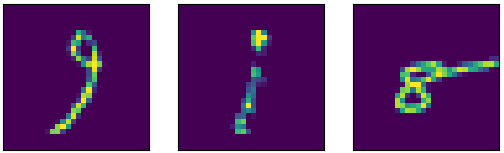
\includegraphics[width=0.5\linewidth]{img/cnn_categorial_cross_non_perm.png}
	\caption{Top three most misclassified digits with the CNN-CEE net}
	\label{fig:cnn}
\end{figure}

The three most misclassified digits of the MLP, shown in figure \ref{fig:mlp}, stand in stark contrast to that.
The left and the right sample seem to be very clearly identifiable.
One problem might be the thickness given that both samples are quite thick.
The middle one is easily identifiable by a human, but is very thin compared to the others, which might be the reason why it was misclassified.
Of course other reasons could have led to this result as well.

\begin{figure}[H]
	\centering
	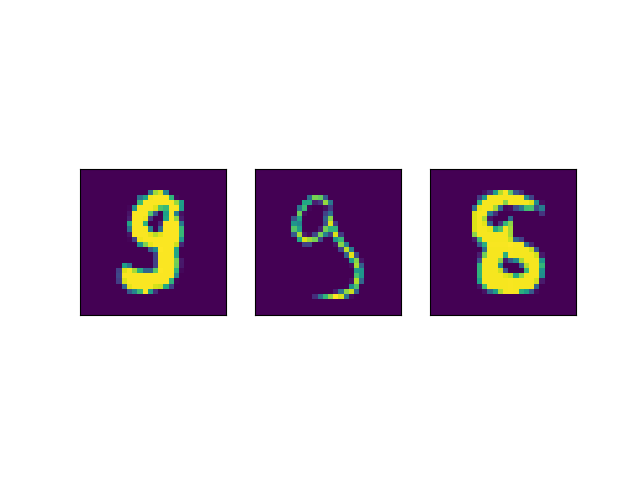
\includegraphics[width=0.5\linewidth]{img/mpl_categorial_cross_non_perm.png}
	\caption{Top three most misclassified digits with the MLP-CEE net}
	\label{fig:mlp}
\end{figure}

\subsection{Evaluation}
\label{evaluation}

In table \ref{table-1} you can see the amount of misclassified samples out of a total of 10000 test samples per experiment.
The rows describes the net type and the columns describe the error function and whether the permuted or the original data set was used.
It is evident, that CNN outperforms the MLP.

Both networks perform best with the cross-entropy error function.
The mean-squared error only slightly worsens the results of the MLP.
The CNN however, performs much worse using the mean squared error.

When looking at the results for the permuted data, we can see that it has a much greater impact on the CNN than on the MLP results.
It almost doubles the misclassified samples with the CNN, but doesn't affect the MLP results significantly.
This effect can be explained by the nature of the convolutional filters.
A convolutional filter \enquote{detects} features by looking at multiple information, in this case multiple pixels, at the same time.
By permutation the data, the feature recognition cannot work properly anymore, because it's important which pixels are next to each other.
The permutation will affect the results of the filters in an unpredictable way.

This problem doesn't occur with a plain MLP net, because every pixel considered individuality.
As long as a pixel is moved to another place consistently over all images, it doesn't affect the behavior at all.


\begin{table}[H]
	\centering
	\begin{tabular}{|l|l|l|l|l|}
		\hline
		& \cellcolor[HTML]{C0C0C0}CEE & \cellcolor[HTML]{C0C0C0}CEE-P & \cellcolor[HTML]{C0C0C0}MSE & \cellcolor[HTML]{C0C0C0}MSE-P \\ \hline
		\cellcolor[HTML]{C0C0C0}MLP & \cellcolor[HTML]{FFFFFF}166 & 178                           & 169                         & 189                           \\ \hline
		\cellcolor[HTML]{C0C0C0}CNN & 77                          & 123                           & 149                         & 221                           \\ \hline
	\end{tabular}
	\caption{Amount of misclassified samples. CEE = cross-entropy error; MSE = mean-squared error, P = permutated sample}
	\label{table-1}
\end{table}

\subsection{Randomness impact}
To determine the possible impact of randomness upon accuracy of the recognition we run same tests again.
The results are shown in table \ref{table-2}.
As you can see, the results don't differ too much from the first runs.
The margin between the misclassified samples seems negligible.


\begin{table}[H]
	\centering
	\begin{tabular}{|l|l|l|l|l|}
		\hline
		& \cellcolor[HTML]{C0C0C0}CEE & \cellcolor[HTML]{C0C0C0}CEE-P & \cellcolor[HTML]{C0C0C0}MSE & \cellcolor[HTML]{C0C0C0}MSE-P \\ \hline
		\cellcolor[HTML]{C0C0C0}MLP & \cellcolor[HTML]{FFFFFF}154 & 160                           & 169                         & 174                           \\ \hline
		\cellcolor[HTML]{C0C0C0}CNN & 88                          & 128                           & 147                         & 216                           \\ \hline
	\end{tabular}
	\caption{Amount of misclassified samples. CEE = cross-entropy error; MSE = mean-squared error, P = permutated sample}
	\label{table-2}
\end{table}

\section{Processing Sequences using LSTM's and GRU's}
\label{sec:seq}
This section deals with using LSTM's and GRU's for natural language processing.
It is split up into two parts one dealing with the generation of text (section \ref{sec:gen}) based on the learned data and the one that handles the translation of text (Section \ref{sec:trans})
\subsection{Generating Text}
\label{sec:gen}
The text generation is based on the \textit{keras}-example code called \textit{lstm\_text\_generation.py}\footnote{\url{https://github.com/keras-team/keras/blob/master/examples/lstm_text_generation.py} ; Visited 04.04.2018}.
In order to evaluate the generation we run the following experiments
\begin{itemize}
\item{Run the example-script as is}
\item{Run the example with different text input}
\item{Run the example with different text input and adjusted parameters to the LSTM}
\item{Run the example with different text input and use a GRU instead of LSTM}
\end{itemize}


TODO: mention sliding window


Also the standard script uses a sequence length of 40 characters. We found that a little short. In order to find a good length we looked up the average sentence length in the english language which is supposed to be 15-20\footnote{\url{http://countwordsworth.com/blog/what-is-a-good-average-sentence-length/} ; Visited 04.04.2018}.
Also the average word length is approximately 5 characters\footnote{\url{https://www.quora.com/Whats-the-average-length-of-English-words} ; Visited 04.04.2018}. Combining that results in 100 characters per sentence ($20 * 5$). We also expect a longer sequence length to improve the generated result, given that LSTM's use historical data well, and short sequences might already have dropped relevant previous context\footnote{\url{http://colah.github.io/posts/2015-08-Understanding-LSTMs/}; Visited 04.04.2018}.

Running the vanilla example script generates very noisy text with a lot of new lines where they are not supposed to be. That is why we decied to write a cleaner for the custom text.

We chose to use all bands of harry potter which are available as txt files on archive.org.
It does contain "noise" in the sense of page numbers, titles which were misread due to ocr etc. We filtered this out with a script.
We also had a few problems with the script aborting due to non-ascii characters being contained in the text, hence we had to drop even more content from the file to work properly.

TODO: abschnitt long term dependencies. france beispiel erwähnen

\subsection{Translating Text}
\label{sec:trans}
\begin{itemize}
\item{Run the example-script as is with french to english translatoin}
\item{Run the example with NL-ENG input}
\item{Run the example with NL-ENG input and adjusted parameters to the LSTM}
\item{Run the example with NL-ENG input and use a GRU instead of LSTM}
\end{itemize}

\section{Learning to calculate from Sequences using RNN}
\label{sec:rnn}


The provided example script tries to teach a RNN to do simple additions by solely providing sequence to sequence string data.
We modified it to do a multiplication, and generate around 270k entries. The training process is quite lengthy, having reached epoch 17 / 35 after 43 hours our Job got cancelled due to a reboot.
We decided 15 Epochs will have to do and saved the model via keras model.save function. This turned out to be a smart decision because after successfull training, a unicode character exception flew which we were able to debug quickly through the pretrained model.







\end{document}